\documentclass[12pt,letterpaper]{article}
\usepackage{fullpage}
\usepackage[top=2cm, bottom=4.5cm, left=2.5cm, right=2.5cm]{geometry}
\usepackage{amsmath,amsthm,amsfonts,amssymb,amscd}
\usepackage{comment}
\usepackage{lastpage}
\usepackage{enumerate}
\usepackage{fancyhdr}
\usepackage{mathrsfs}
\usepackage{xcolor}
\usepackage{graphicx}
\usepackage{subcaption}
\usepackage{listings}
\usepackage{hyperref}
\usepackage{enumitem}

\hypersetup{%
  colorlinks=true,
  linkcolor=blue,
  linkbordercolor={0 0 1}
}
 
\renewcommand\lstlistingname{Algorithm}
\renewcommand\lstlistlistingname{Algorithms}
\def\lstlistingautorefname{Alg.}

\lstdefinestyle{Python}{
    language        = Python,
    frame           = lines, 
    basicstyle      = \footnotesize,
    keywordstyle    = \color{blue},
    stringstyle     = \color{green},
    commentstyle    = \color{red}\ttfamily
}

\setlength{\parindent}{0.0in}
\setlength{\parskip}{0.05in}

% Edit these as appropriate
\newcommand\course{6.869 Advances in Computer Vision}
\newcommand\hwnumber{1}                  % <-- homework number
\newcommand\name{Felipe Moreno}
\newcommand\collaborators{Collaborators: None}

\pagestyle{fancyplain}
\headheight 35pt
\lhead{\name}
\lhead{\name\\ \collaborators}
\chead{\textbf{\Large Final Project Report }}
\rhead{\course \\ \today}
\lfoot{}
\cfoot{}
\rfoot{\small\thepage}
\headsep 1.5em

\begin{document}
	
\section{Abstract}
Currently, Jibo, the original social robot, lacks plenty of functionalities after its company Jibo, Inc abruptly shut down in 2018. Jibo is currently used by researchers in the Personal Robots Group in the MIT Media Lab, to conduct user studies in the field of social robotics. In this project, we develop 3D reconstruction functionality and object detection on Jibo. The motivation is that currently Jibo lacks the functionality to interact with the environment and to have a semantic understanding of its surroundings. In this project we the solve depth estimation problem using the stereo reconstruction from Jibo's two frontal cameras.

\begin{figure}[h]
	\centering
	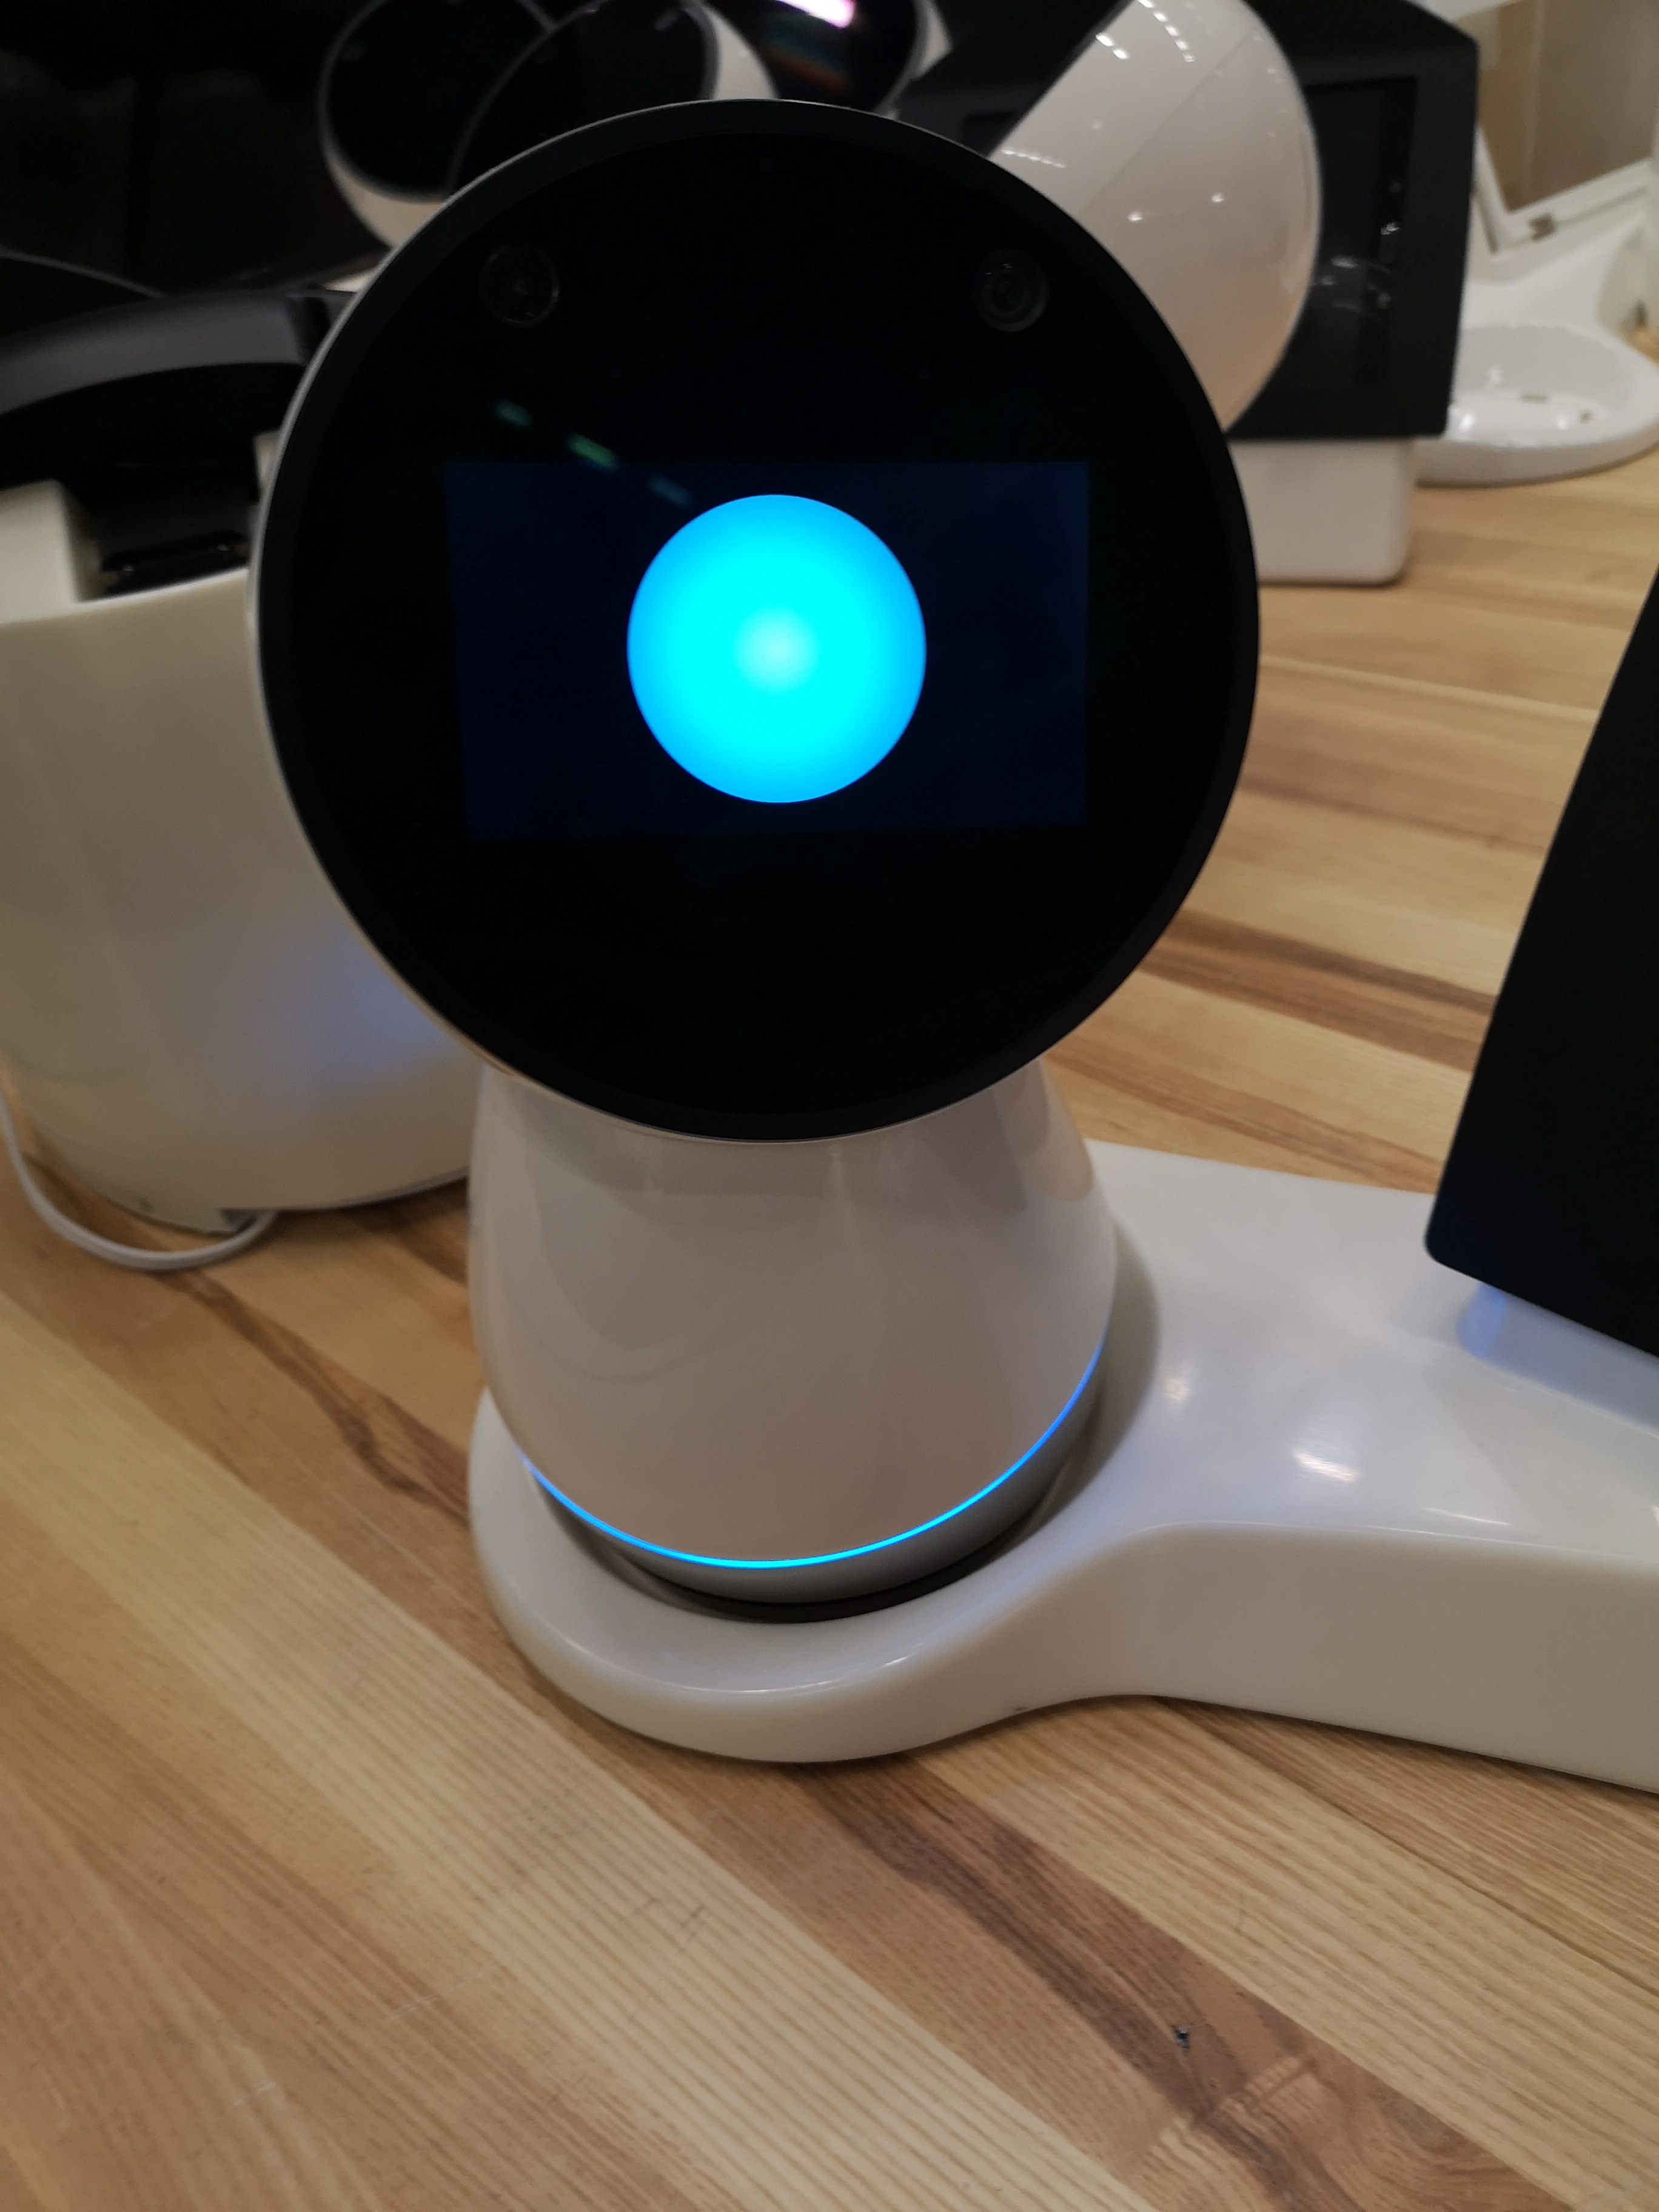
\includegraphics[width=0.3\linewidth]{./images/jibo.jpg}
	\caption{Jibo robot}
\end{figure}

\section{Introduction}
The Jibo robot was created with the goal to become the first social robot for the home. By the time the company Jibo, Inc. shutoff in 2018, due to a series of mistakes and the ruthless competition with smart speakers such as Alexa and Google home with costs under 50\$ as compared to Jibo which sold for a price of \$899 at the time, only an SDK with limited functionality was released to developers to produce third-party apps. Since then Jibo has been kept alive by researchers and, in particular, the MIT Media Lab Personal Robots Group which to this day uses Jibo to deploy user studies on Social Robotics.

% What capabilities does Jibo have
Jibo features a peculiar design. It is a statically fixed to the ground i.e it does not have legs to move, yet its torso has 360$\deg$ of freedom to rotate around and it's head the ability to look upwards and downwards. For that reason, it is great interest for Jibo to have an understanding of its environment.  Future studies plan to have Jibo deployed on living spaces where it can extract meaningful information from its surroundings to better engage with the user. Jibo has two frontal cameras as shown in Figure(\ref{camera_setup}).

\begin{figure}[ht]
	\begin{tabular}[c]{ccc}
		\begin{subfigure}[c]{0.3\linewidth} 
			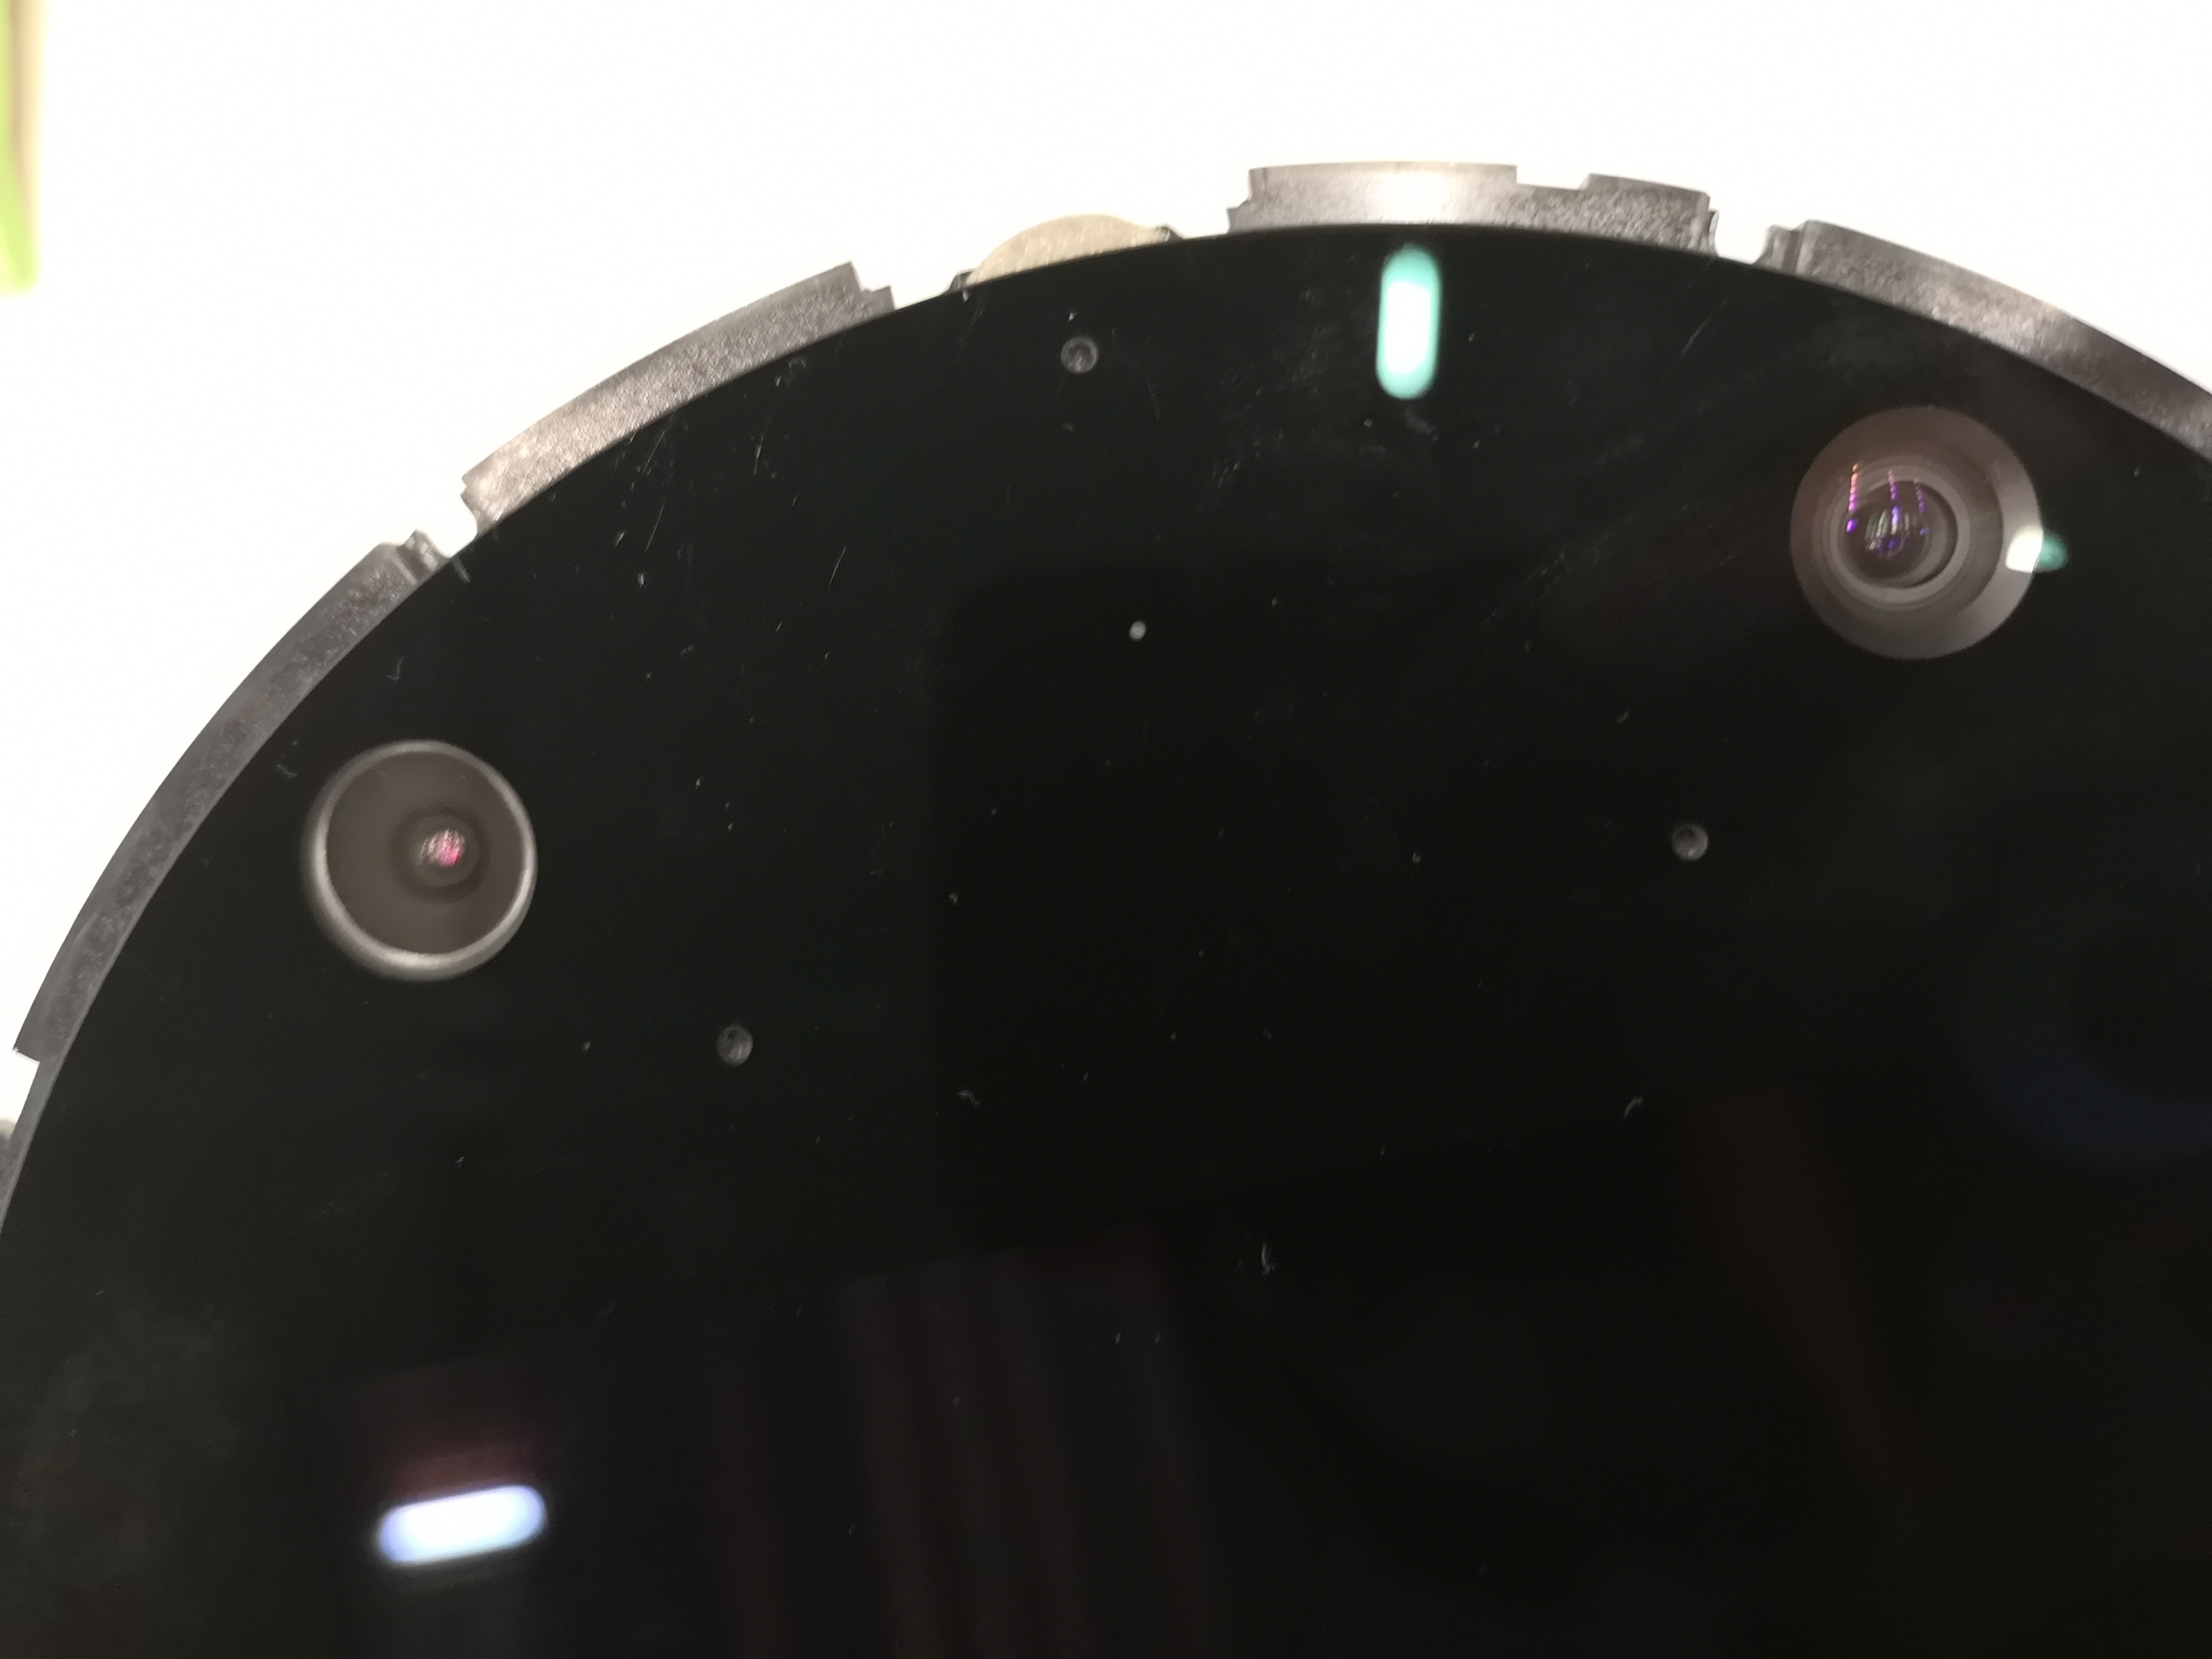
\includegraphics[width=\linewidth]{./images/cameras.jpg}
			\subcaption{Jibo frontal cameras. Left is a narrow lens camera and right is a wide lens.}
		\end{subfigure}&
		\begin{subfigure}[c]{0.3\linewidth}
			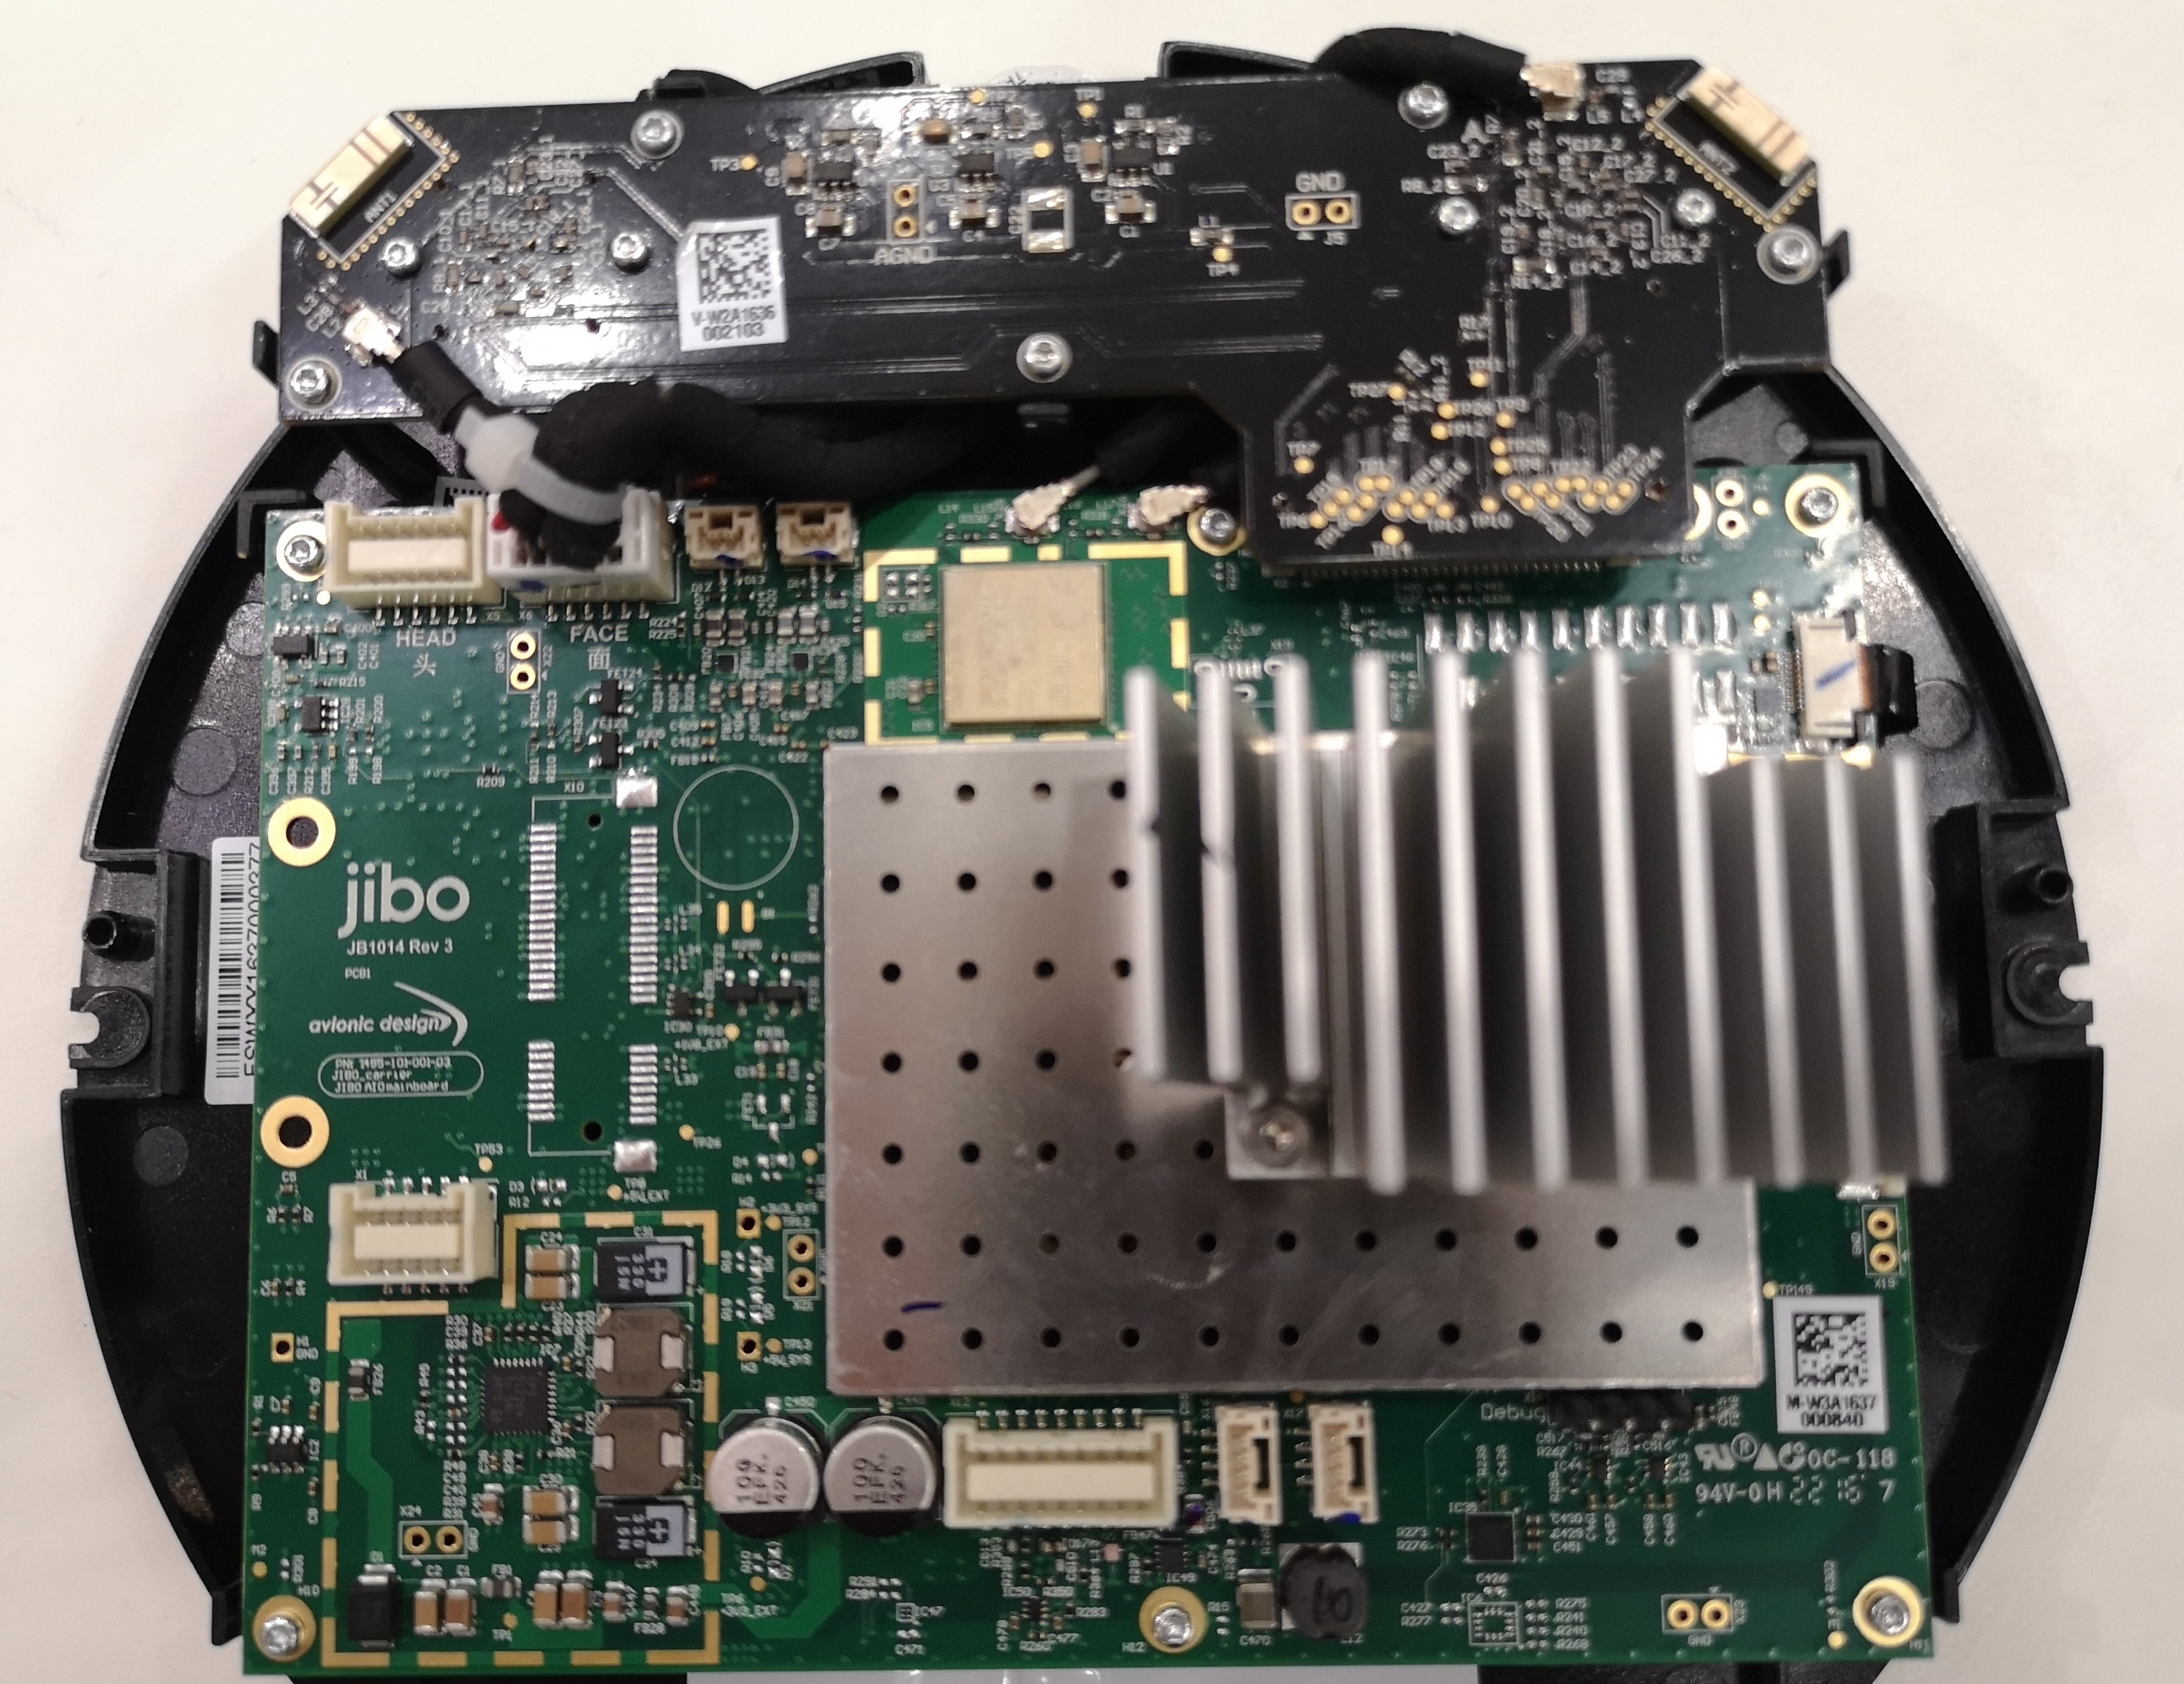
\includegraphics[width=\linewidth]{./images/camera_board_front.jpg}
			\subcaption{Jibo camera board inside view}
		\end{subfigure}&
		\begin{subfigure}[c]{0.3\linewidth}
			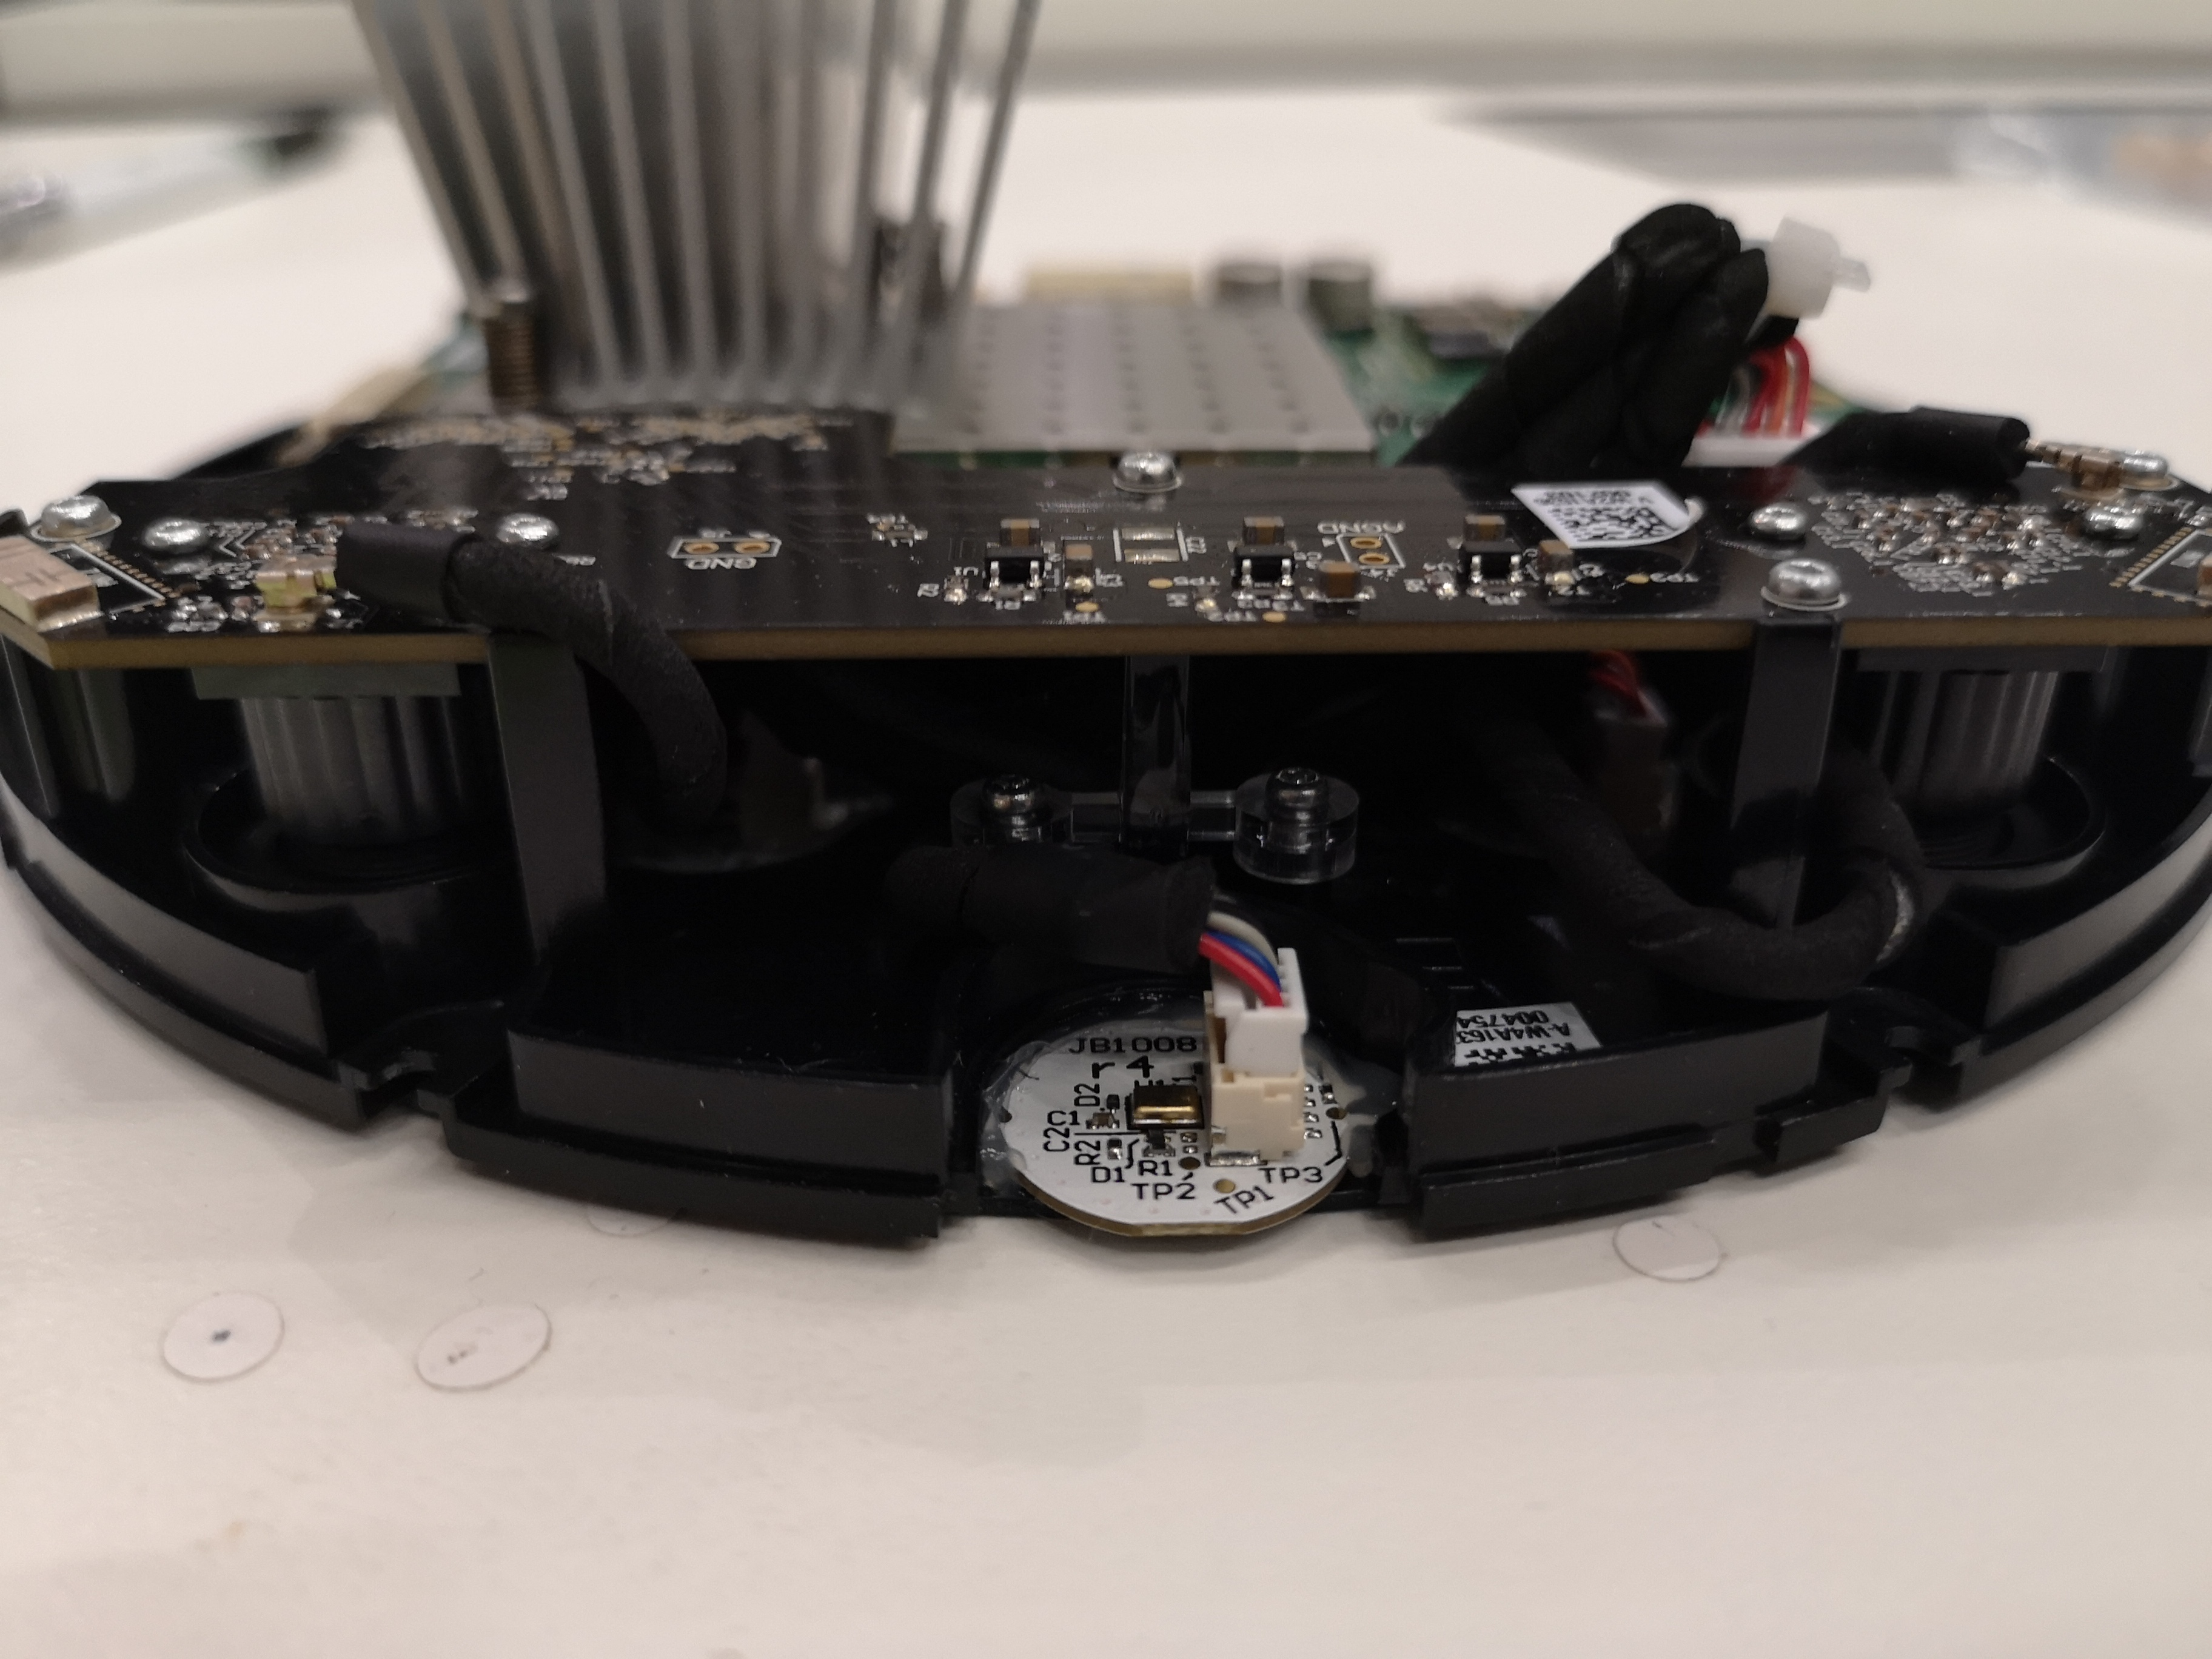
\includegraphics[width=\linewidth]{./images/camera_board_side.jpg}
			\subcaption{Jibo camera board side view}
		\end{subfigure}
	\end{tabular}
	\caption{Jibo camera board setup}
	\label{camera_setup}
\end{figure}

In this work, the focus is the integration of depth perception for environment understanding.

\section{Related Work}
In the literature review, we explored multiple approaches to having Jibo reconstruct the depth maps of its surrounding environment in real time. We reviewed many possible methods using both cameras or a single camera.  We looked at to recover intrinsic from a single image from  \cite{tappen2003recovering}. We also explored the idea of using video to extract depth maps as done in \cite{larsen2006simplified} and \cite{koch1998multi}. We looked into the deep learning literature to understand data driven ways to approach the problem as done in \cite{gur2019single}. 

However these approaches fail to be ideal for our problem - real-time depth estimation. This problem has been extensively studied in robotics with stereography. We choose this approach because of its ease of implementation and the ability to make use of the robot's default hardware.

Lastly we looked at some algorithms for computing the disparity maps between stereo images as described in which uses a Graph Cuts algorithm to achieve high performance \cite{tappen2003comparison}. But we decide to go with using SURF \cite{bay2006surf} since it is a fast and high performance algorithm for keypoint matching which is very appropriate to use in our application. Since the robot, is expected to estimate depths in real time performance is one of our main concerns. Its worth noting that SURF is a patented algorithm, but it can be freely used for research purposes which is our academic goal.

We also explored the possibility of replacing the cameras for two cameras of the same type. As it turns out, the platform that the robot runs expects the cameras to be the given ones and replacing the cameras would be a task that needs to also be handled at robot's architecture level.

\section{Approach}
As expected by a company that abruptly shutoff, the Jibo documentation was very obscure and hard to dig into. Our first approaches to the problem were optimistic about being able to find a solution without completely knowing the actual hardware of the robot nor the software running on it. We were able to get images from the camera using API calls yet were uninformed about any processing done on the images extracted through the API calls. The resulting images looked as show in Figure(\ref{raw_captures}).

\begin{figure}[ht]
	\centering
	\begin{subfigure}[c]{0.4\linewidth} 
		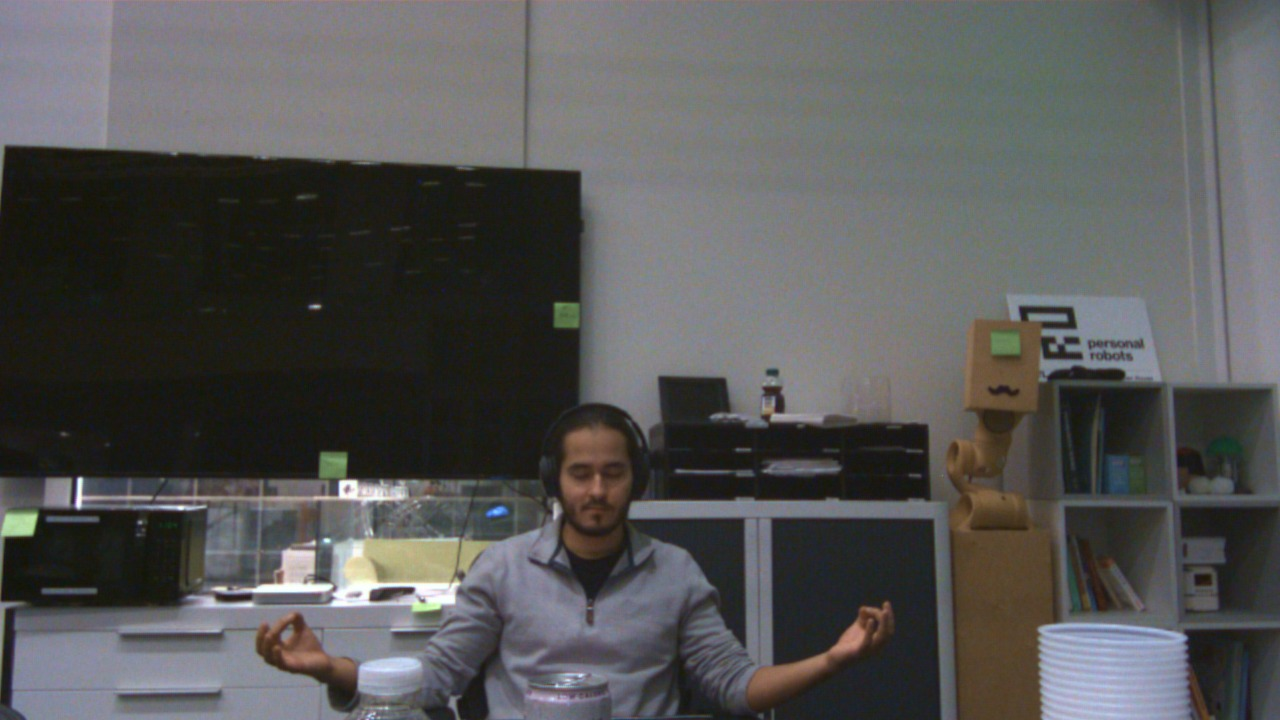
\includegraphics[width=\linewidth]{./images/pinhole_9.png}
		\subcaption{Capture made with the narrow lens camera.}
	\end{subfigure}
	\begin{subfigure}[c]{0.4\linewidth}
		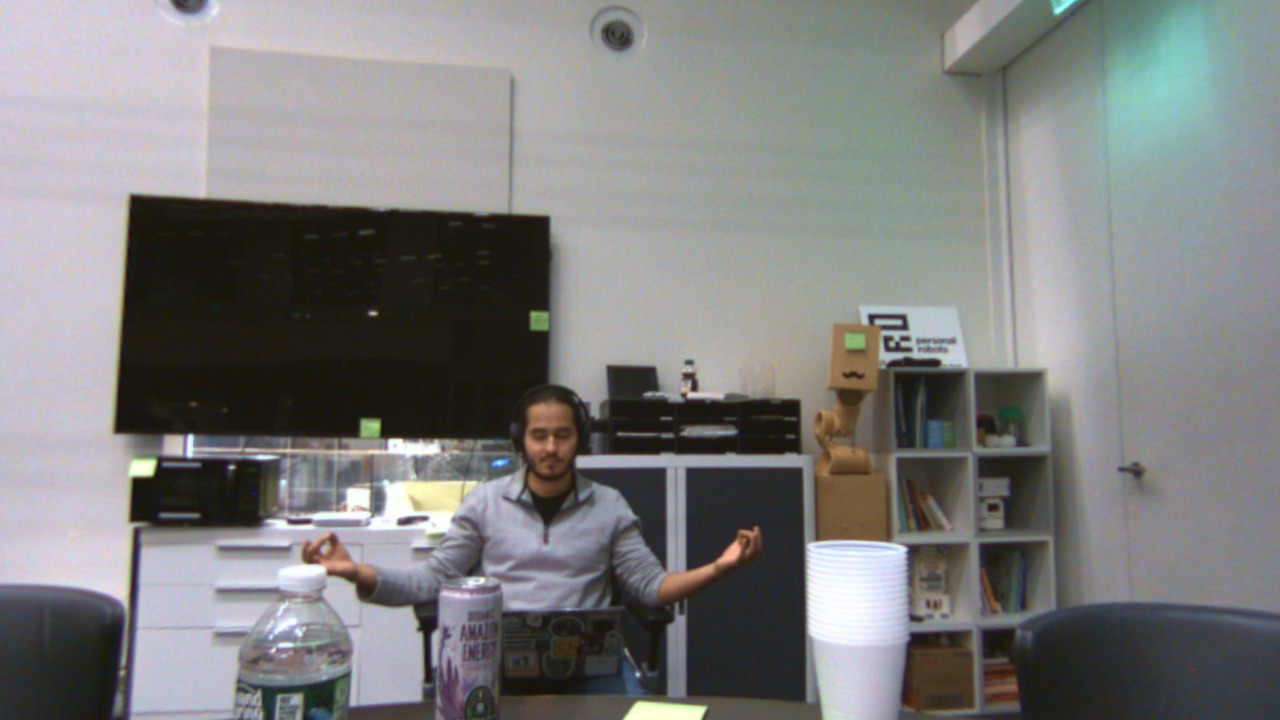
\includegraphics[width=\linewidth]{./images/fisheye_9.png}
		\subcaption{Capture made with the wide lens camera.}
	\end{subfigure}
	\caption{Raw camera captures}
	\label{raw_captures}
\end{figure}

Digging through the documentation, we found the part numbers for both of the robot's cameras. We discovered that their field of views were $82^\circ$ and $131^\circ$. The documentation referred to the wide lens camera as a `fisheye camera' as well as a `wide lens camera'. For this reason, we tried different camera calibration approaches on this camera until we found good results.

For camera calibration we used the chessboard detect corners approach to compute the intrinsic of each camera. We then undistort the images and crop the region of interest. With a pinhole camera model calibration method we achieve good results for the narrow lens camera, as show in Figure(\ref{pinhole_calibration}).

\begin{comment}	
	\begin{figure}[ht]
		\centering
		\begin{subfigure}[c]{0.4\linewidth} 
			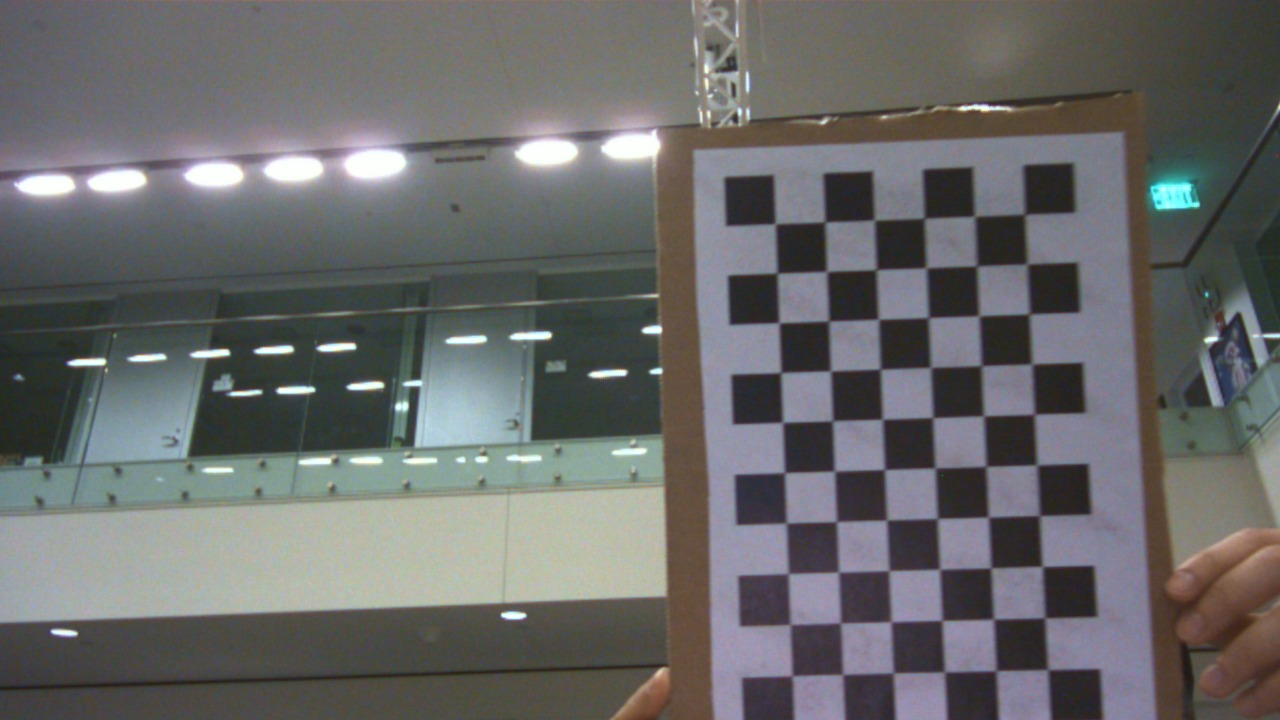
\includegraphics[width=\linewidth]{./images/pinhole_raw_calibration.png}
			\subcaption{Raw narrow lens image}
		\end{subfigure}
		\begin{subfigure}[c]{0.3\linewidth}
			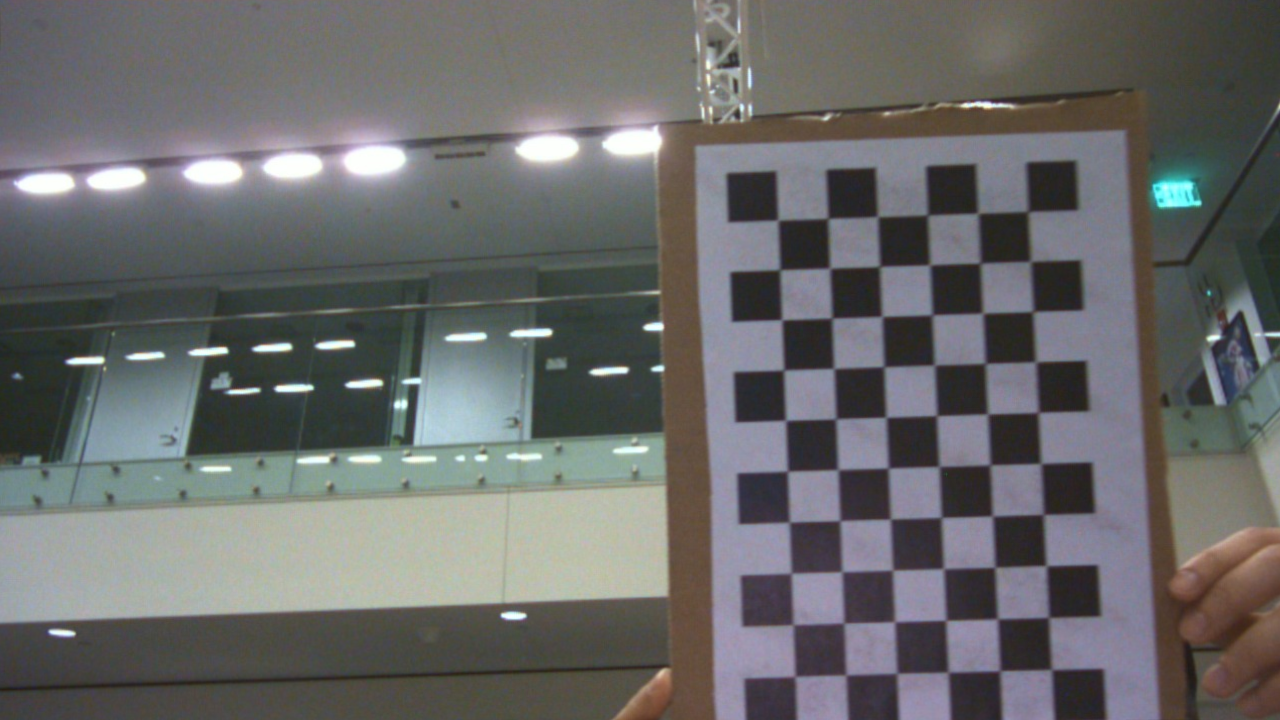
\includegraphics[width=\linewidth]{./images/pinhole_undistorted_calibration.png}
			\subcaption{Undistorted narrow lens image}
		\end{subfigure}
		\caption{Narrow lens calibration images}
		\label{pinhole_calibration}
	\end{figure}
\end{comment}

Calibrating the wide lens camera was much more difficult. First attempt was to calibrate using the fisheye camera model or the pinhole camera model which gave terrible results as shown in Figure (\ref{fisheye_calibration}). The rational camera model is described, in the OpenCV documentation as computing 8 distortion coefficients instead of the standard 5, gives much better results although we still find some distortion towards the sides of the image. The solution we found was to increase the number of calibration images, and add more diversity to the set.

	\begin{figure}[ht]
	\begin{tabular}[c]{ccc}
		\begin{subfigure}[c]{0.3\linewidth} 
			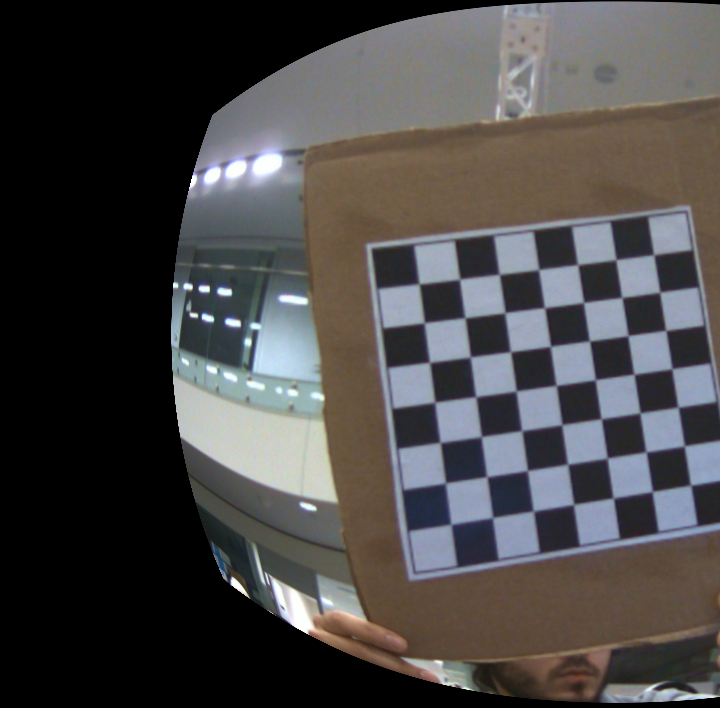
\includegraphics[width=\linewidth]{./images/fisheye_fisheye_calibration.png}
			\subcaption{Undistorted image using the fisheye camera model.}
		\end{subfigure}&
		\begin{subfigure}[c]{0.3\linewidth}
			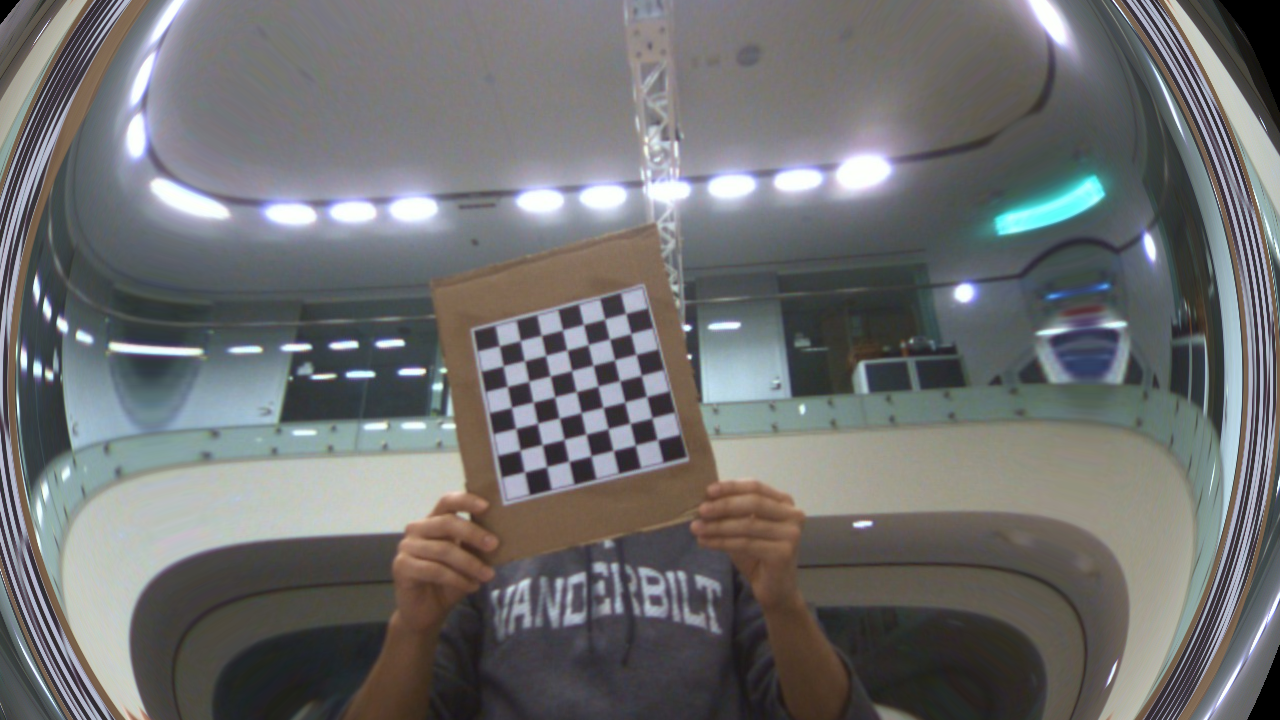
\includegraphics[width=\linewidth]{./images/fisheye_pinhole_calibration.png}
			\subcaption{Undistorted image using the pinhole camer model.}
		\end{subfigure}&
		\begin{subfigure}[c]{0.3\linewidth}
			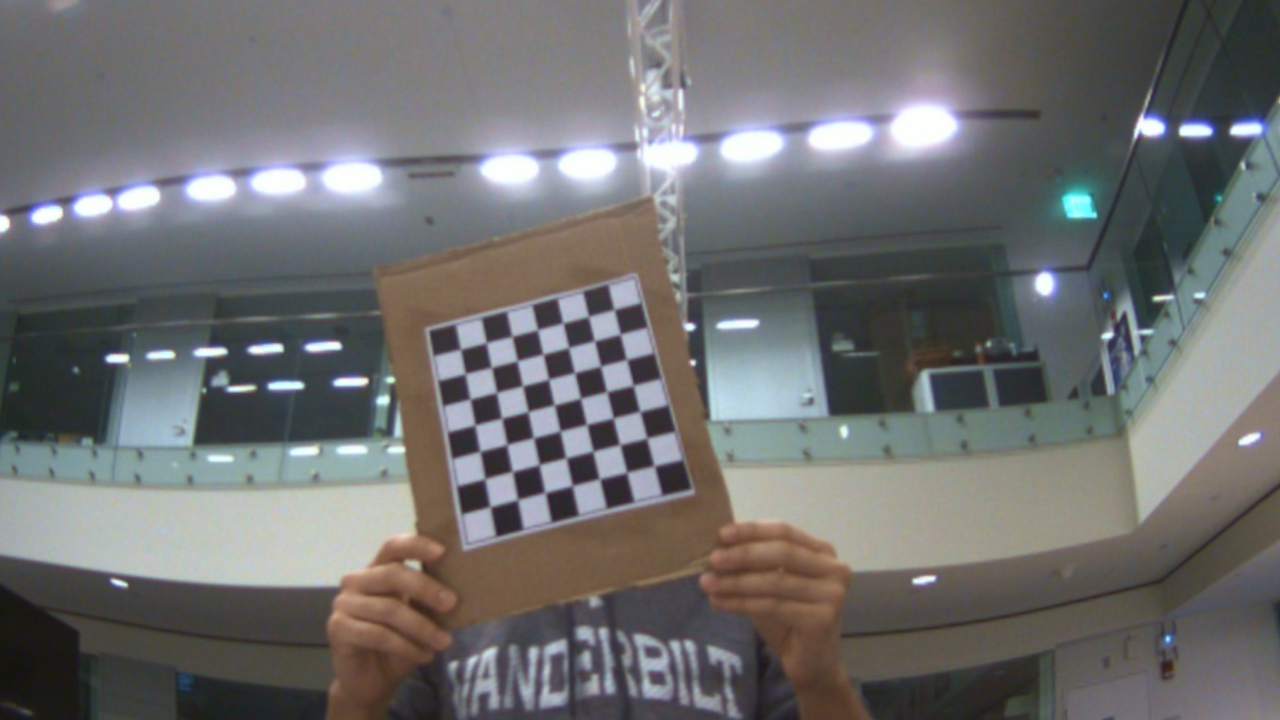
\includegraphics[width=\linewidth]{./images/fisheye_rational_calibration.png}
			\subcaption{Undistorted image using the rational camera model.}
		\end{subfigure}
	\end{tabular}
	\caption{Difficulties in calibrating the wide lens camera.}
	\label{fisheye_calibration}
\end{figure}

\begin{comment}
	\begin{figure}[htb]
		\centering
		\begin{subfigure}[c]{0.4\linewidth} 
			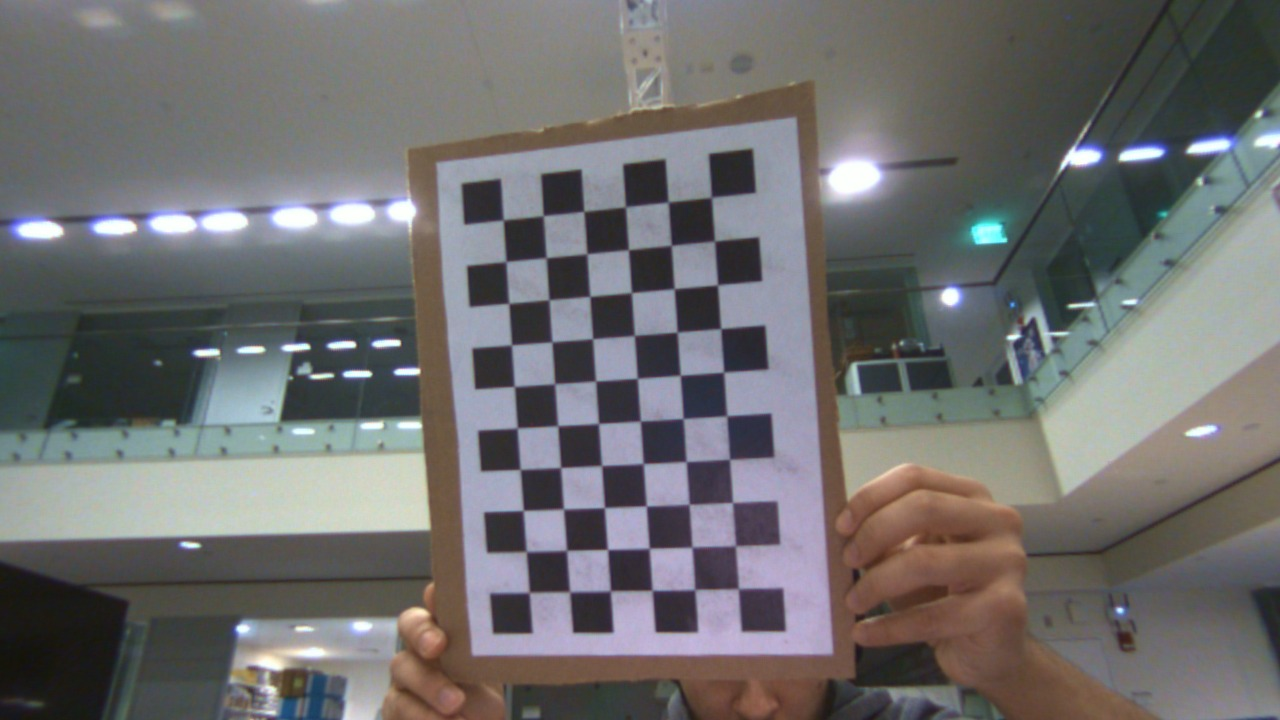
\includegraphics[width=\linewidth]{./images/fisheye_raw_calibration_2.png}
			\subcaption{Raw wide lens image}
		\end{subfigure}
		\begin{subfigure}[c]{0.4\linewidth}
			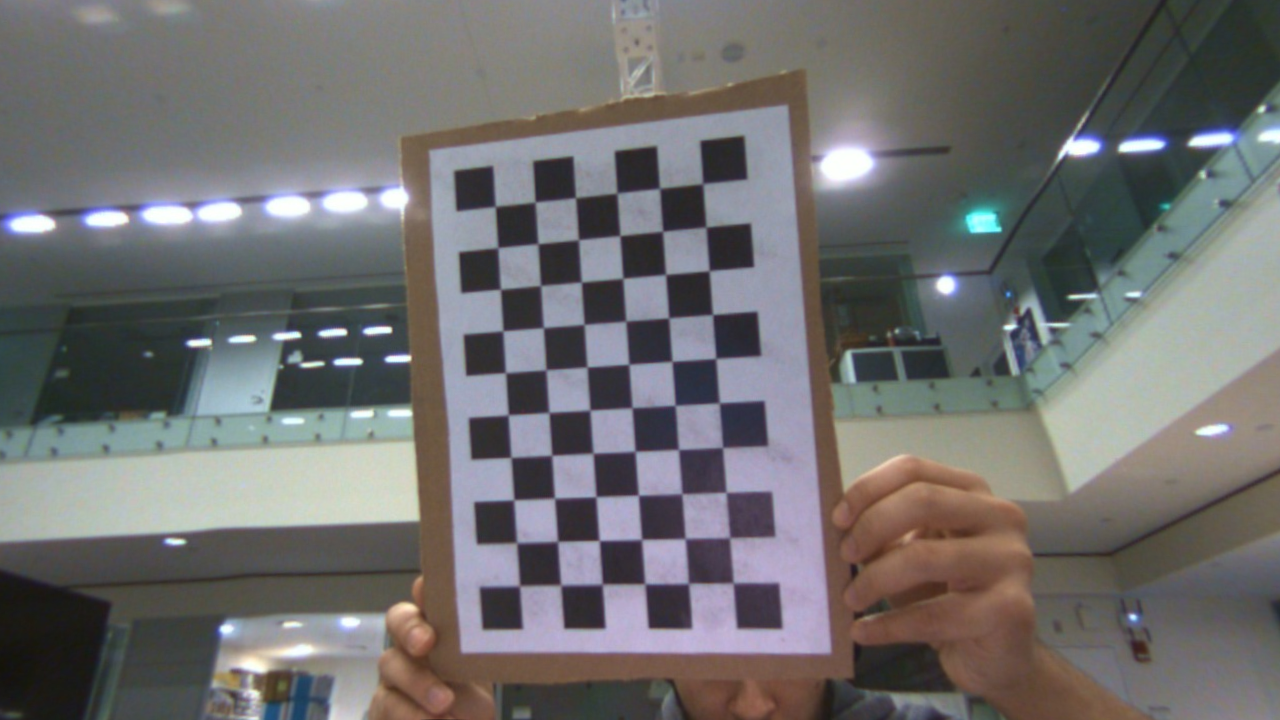
\includegraphics[width=\linewidth]{./images/fisheye_calibrated.png}
			\subcaption{Undistorted wide lens image}
		\end{subfigure}
		\caption{Wide lens undistorted image results.}
		\label{wide_undistortion}
	\end{figure}
\end{comment}

We then proceeded with the next stage of the problem, image rectification. We decided to use an asymmetrical chess board to avoid the epipolar lines to be detected in two different orientations. With this step, we achieve the results of a rectified image as shown in Figure (\ref{keypoint_matching}). 

\begin{figure}[htb]
	\centering
	\begin{subfigure}[c]{0.4\linewidth} 
		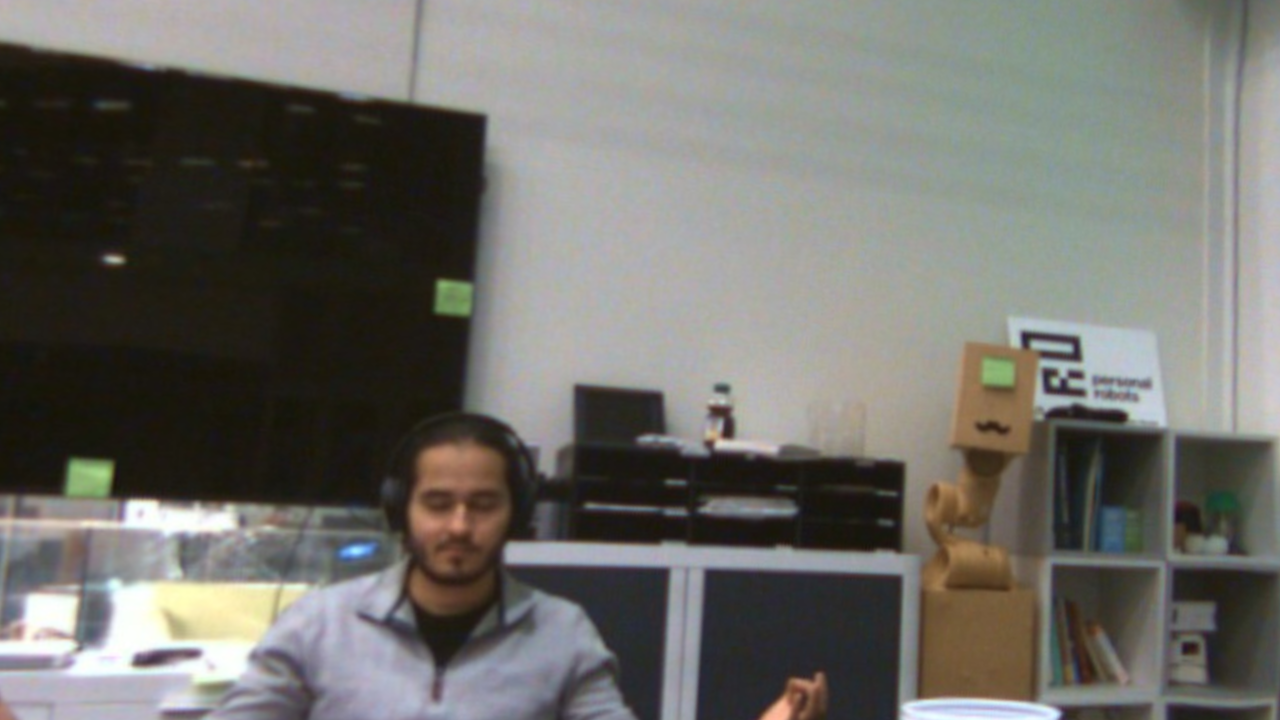
\includegraphics[width=\linewidth]{./images/stereo_calibrated_left.png}
		\subcaption{Wide lens camera rectification result.}
	\end{subfigure}
	\begin{subfigure}[c]{0.4\linewidth}
		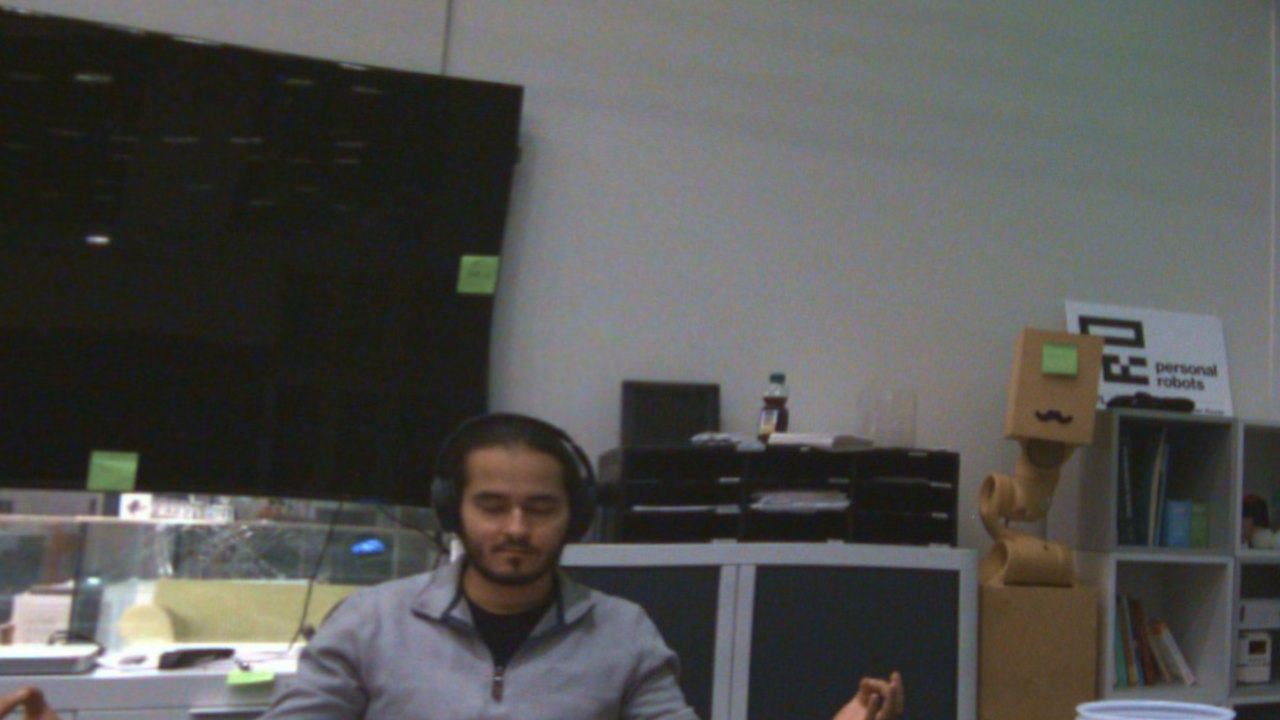
\includegraphics[width=\linewidth]{./images/stereo_calibrated_right.png}
		\subcaption{Narrow lens camera rectification result.}
	\end{subfigure}
	\caption{Rectification results}
	\label{rectification_results}
\end{figure}

Now that we have rectified images, we proceeded to find matching keypoints between the two rectified images. We used SURF algorithm to detect the matching keypoints, we then used Lowes distance ration method to filter out bad matches. These results look like Figure().

\begin{figure}[hbt]
	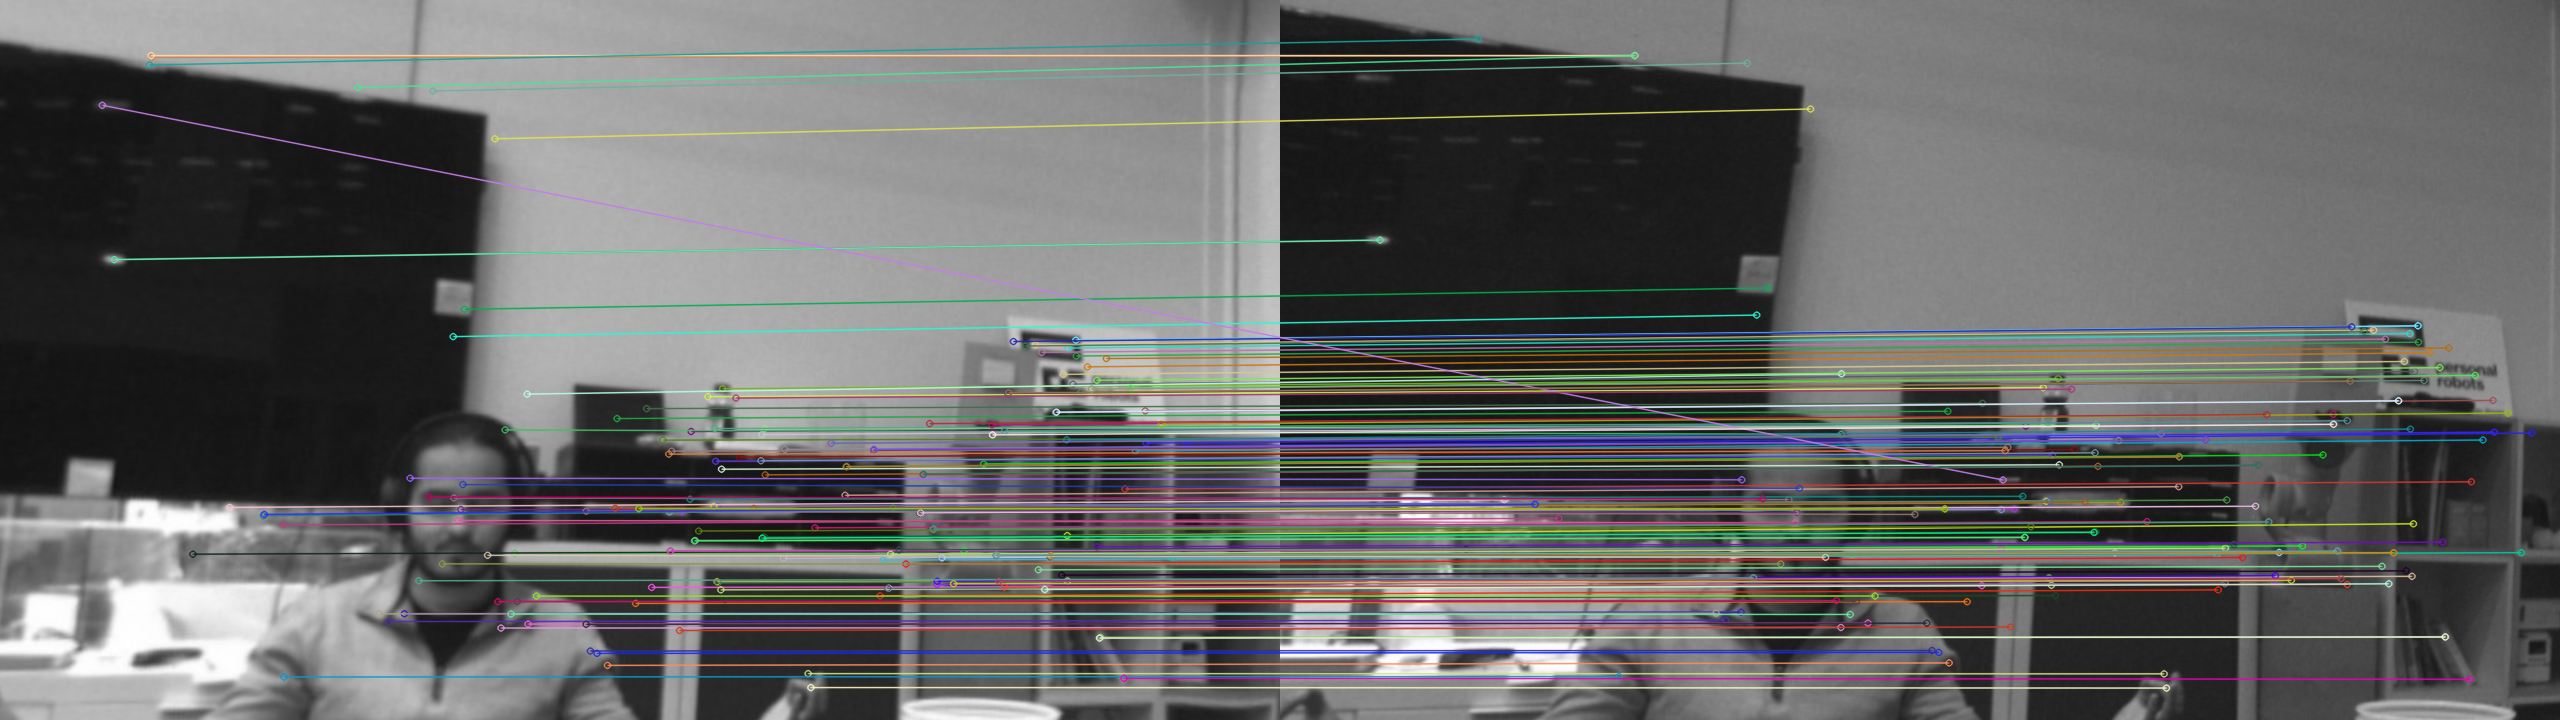
\includegraphics[width=\linewidth]{./images/eval2_matches_9.png}
	\caption{Keypoint matching pairs}
	\label{keypoint_matching}
\end{figure}

From the disparity maps, we can triangulate the depth of every keypoint using the focal length of the cameras and the baseline distance between them.

\section{Experimental Results}

For system validation, we measured 10 objects in the environment at various distances from the robot. We then predict the depths for all of the objects in question by averaging all the keypoints in each object. Predicted depths are reported in Figure(\ref{depth_results}).

\begin{figure}[htb]
	\centering
	\begin{subfigure}[c]{0.4\linewidth} 
		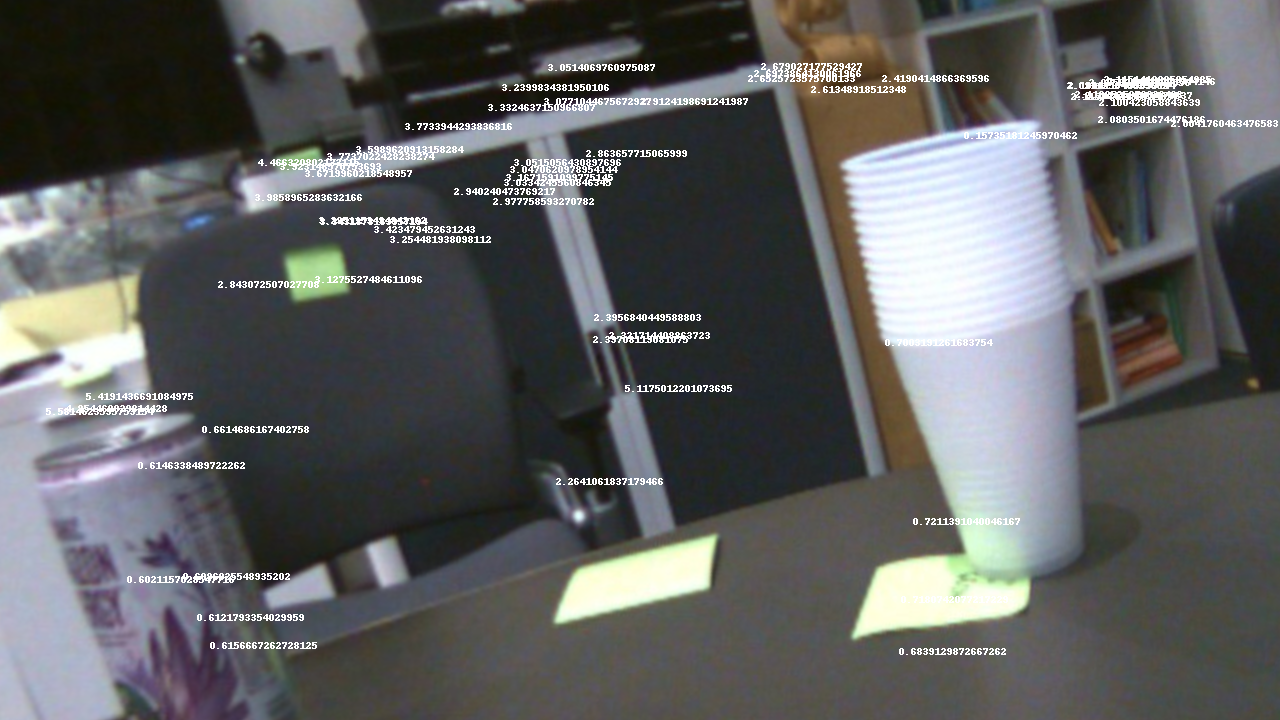
\includegraphics[width=\linewidth]{./images/depth_results_8.png}
		\subcaption{}
	\end{subfigure}
	\begin{subfigure}[c]{0.4\linewidth}
		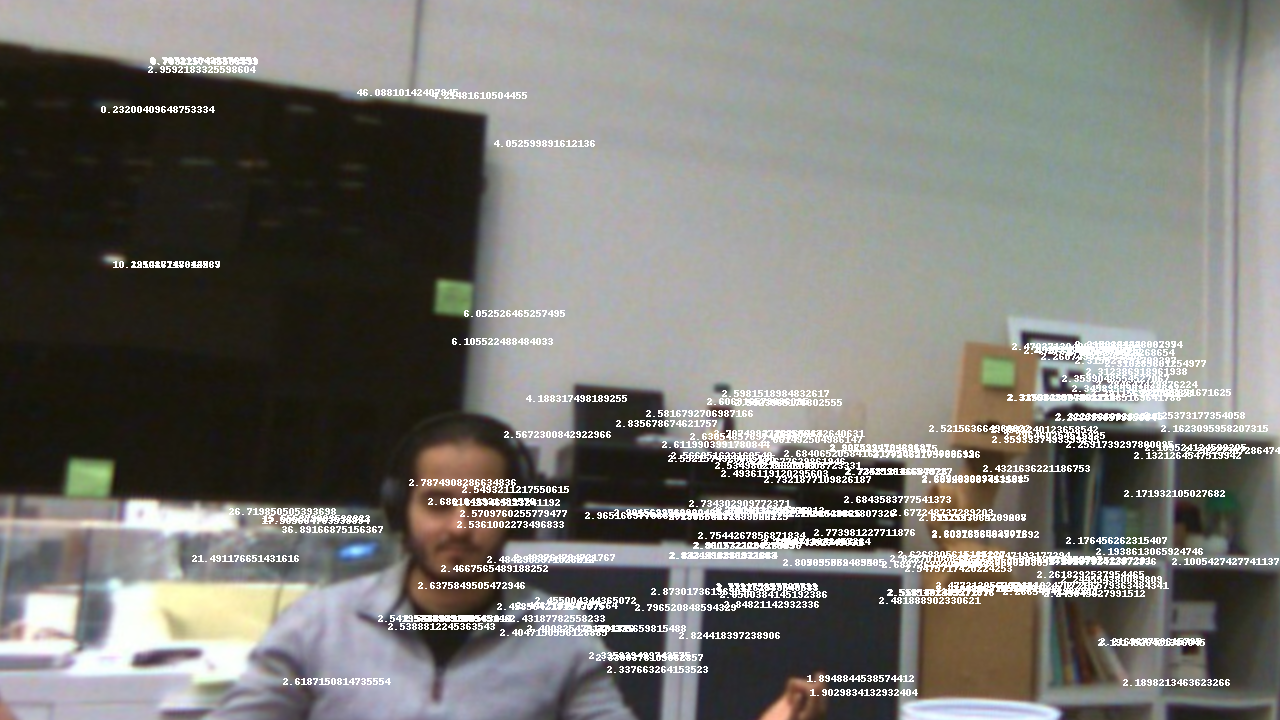
\includegraphics[width=\linewidth]{./images/depth_results2_9.png}
		\subcaption{}
	\end{subfigure}
	\caption{Rectification results}
	\label{depth_results}
\end{figure}

For each object, we calculated the error as the absolute difference between the ground truth and the prediction. We clustered the objects into 3 range distances from the robot (0.5m, 1.5m), [2.5m, 3.5m), [3.5m, 4.5m). We report the mean errors for each range in Figure(\ref{errors}). We observe high accuracy for nearby objects, but increasing errors the farther the object is from the robot.

\begin{figure}[h]
	\centering
	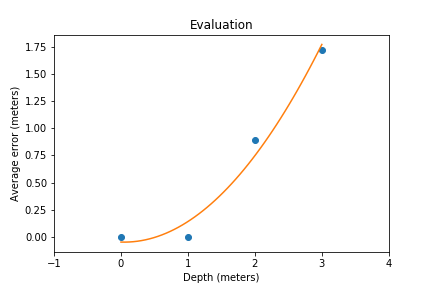
\includegraphics[width=0.7\linewidth]{./images/errors.png}
	\caption{Measured error }
\end{figure}

\section{Conclusion}
The proposed method is successful at measuring with high accuracy objects nearby to the robot. Nevertheless, far away object depths, can't be reliable determined. For future work, we propose using belief propagation to further refine predictions based on past observations. Also future work will hope to incorporate the robot's semantic understanding of the environment with depth perception and all of this functionality to run natively on the robot. Currently, these results are obtained on fetched images from the robot. There is still work to be done at the architecture level to allow installation of libraries and packages in the robot that will allow for this project to run on the robot.

\section{References}
\bibliographystyle{plainnat}
%\bibliographystyle{plain}
\bibliography{references}

\end{document}


